% coherence_modeling.tex
% Self-contained deep-dive on probabilistic modeling of the logical coherence of
% an LLM response. Compile: pdflatex coherence_modeling.tex (run twice).
%
% Companion to docs/ideation/research_plan.md. All numeric marginals / Z / MAP
% values in Sections 5-6 are EXACT (brute-force over 2^16 worlds) for the model
% defined in Section 3; they were produced by the accompanying reference solver.

\documentclass[11pt]{article}

\usepackage[margin=1in]{geometry}
\usepackage{amsmath}
\usepackage{amssymb}
\usepackage{enumitem}
\usepackage{xcolor}
\usepackage{soul}
\usepackage{booktabs}
\usepackage{array}
\usepackage[numbers,square]{natbib}
\usepackage{tikz}
\usetikzlibrary{arrows.meta,positioning,calc,backgrounds,fit,shapes.geometric}
\usepackage[colorlinks=true,urlcolor=blue!60!black,linkcolor=blue!60!black,
            citecolor=blue!60!black]{hyperref}

% --- atomic-unit highlight palette (roles in the worked example) ---
\definecolor{cChain} {RGB}{210,228,248}   % causal / prerequisite backbone
\definecolor{cEvid}  {RGB}{215,236,219}    % evidence
\definecolor{cEquiv} {RGB}{226,221,243}    % restatement / equivalence
\definecolor{cConflA}{RGB}{248,205,205}    % contradiction side A
\definecolor{cConflB}{RGB}{249,222,229}    % contradiction side B
\definecolor{cHold}  {RGB}{250,219,180}    % resolving holding (concession)

\sethlcolor{cChain}
\newcommand{\fu}[3]{{\sethlcolor{#1}\hl{#2}}\,\textsuperscript{\textbf{\scriptsize #3}}}

% shared tikz styles
\tikzset{
  >={Stealth[length=2.5mm]},
  unit/.style={draw,rounded corners,minimum width=10mm,minimum height=7mm,
               inner sep=1pt,font=\footnotesize\bfseries,fill=cChain},
  evid/.style={unit,fill=cEvid,draw=green!55!black},
  equivn/.style={unit,fill=cEquiv,draw=violet!55!black},
  conflA/.style={unit,fill=cConflA,draw=red!55!black},
  conflB/.style={unit,fill=cConflB,draw=red!45!black},
  hold/.style={unit,fill=cHold,draw=orange!70!black,very thick},
  coh/.style={draw,rounded corners,minimum width=11mm,minimum height=8mm,
              inner sep=1pt,font=\small\bfseries,fill=orange!25,
              draw=orange!70!black,very thick},
  prereq/.style={->,blue!70!black,thick},
  equivedge/.style={<->,violet!70!black,thick},
  invalid/.style={->,red!75!black,dashed,thick},
  resolve/.style={->,orange!80!black,thick},
  factor/.style={-,gray!55,dotted,thick},
}

\title{Probabilistic Modeling of the Logical Coherence of LLM Responses\\
       \large Two-Layer Relations, Markov Networks vs.\ Markov Logic,\\
       and Coherence Scoring --- a Deep Dive}
\author{FactReasoner --- Ideation}
\date{\today}

\begin{document}
\maketitle

\begin{abstract}
\noindent
We deepen the research plan for measuring the \emph{logical coherence} of an
LLM-generated response (as opposed to its factuality). The response is decomposed into
atomic claims; \emph{inter-claim} relations are mined and assigned confidences; a
probabilistic model over claims and relations is built; and a single coherence score is
read out by inference. This document (i) develops the two-layer relation taxonomy
(discourse sense $\to$ inferential coupling); (ii) works the two most promising models ---
the undirected pairwise \textbf{Markov Random Field} (the FactReasoner construction, reused)
and the \textbf{Markov Logic Network} --- rigorously and side by side; (iii) analyzes all
applicable scoring methods and computes them \emph{exactly} on a new, deliberately
intricate worked example that combines a plausible causal chain, an \emph{unresolved}
contradiction, and a \emph{resolved} (conceded) tension. A key modeling finding: for
atom$\leftrightarrow$atom coherence the \emph{with-priors} factor variant already present in
\texttt{assessor.py} is the correct choice, and a reified coherence node plus the
partition-function ratio give the cleanest global scores.
\end{abstract}

\tableofcontents

% =====================================================================================
\section{Setup and notation}
\label{sec:setup}

A response $y$ is decomposed (reusing FactReasoner's atomizer + decontextualizing reviser)
into atomic units $A=\{a_1,\dots,a_n\}$, each a binary random variable: $a_i=1$ ("holds")
or $a_i=0$. We mine a set of directed inter-atom relations
$R=\{r_{ij}=(a_i,a_j,\tau_{ij},p_{ij})\}$, where $\tau_{ij}$ is the relation type and
$p_{ij}\in[0,1]$ its confidence/strength (Section~\ref{sec:conf}). The goal is a
\emph{Logical Coherence Score} $\mathrm{LCS}(y)\in[0,1]$ plus per-atom / per-relation
diagnostics. This reuses the objects in \texttt{src/fact\_reasoner/}: \texttt{FactGraph}
(\texttt{Node}/\texttt{Edge}, where \texttt{Edge.link="atom\_atom"} is already permitted),
\texttt{MarkovNetwork} (UAI serialization), and Merlin for inference.

Two failure modes must be captured, both drawn from \texttt{docs/ideation/*.pdf}:
\textbf{(1) weak inferential links} (true atoms, tenuous asserted relations) and
\textbf{(2) internal contradiction / position invalidation} (a later atom retracts or
conflicts with an earlier one). Crucially, coherence is \emph{order-sensitive}: the
\emph{R v Renda} example (\texttt{example-5}) shows the same facts can be coherent or not
depending only on arrangement.

% =====================================================================================
\section{The two-layer relation taxonomy}
\label{sec:taxonomy}

We separate what the classifier is good at naming (a \emph{discourse} sense) from what the
probabilistic model needs (an \emph{inferential coupling}).

\subsection{Layer B --- discourse sense (interpretable label)}
Grounded in the \textbf{PDTB 3.0} four top-level senses \citep{pdtb3,pdtb2} and
\textbf{RST} \citep{rst}; \textbf{SDRT} \citep{sdrt} supplies the graph (not tree) view and
a formal "maximize coherence" notion. Layer B is what shallow discourse parsers
(\textbf{DiscoPrompt} \citep{discoprompt}, connective-prediction) actually output.

\begin{center}\small
\begin{tabular}{@{}p{2.4cm}p{5.1cm}cp{4.4cm}@{}}
\toprule
\textbf{PDTB top} & \textbf{Sub-senses used here} & \textbf{Dir.?} & \textbf{Typical Layer-A map}\\
\midrule
Contingency & Cause-Effect, Effect-Cause, Evidence, Condition & yes & \textsc{entail} (graded)\\
Temporal    & Precedence, Succession, Synchrony & yes & weak/\textsc{none} + order constraint\\
Comparison  & Contrast, Concession & yes & \textsc{contradict}; Concession $=$ \emph{resolved} tension\\
Expansion   & Elaboration, Restatement, Instantiation/Subsumption & mixed & \textsc{entail}/\textsc{equiv}\\
\bottomrule
\end{tabular}
\end{center}

\subsection{Layer A --- inferential coupling (drives the model)}
A small set matching FactReasoner's existing NLI edge types, so the factor machinery is
reused verbatim:
\begin{itemize}[leftmargin=*,nosep]
  \item \textsc{entail} ($a_i\!\Rightarrow\! a_j$): source true makes target true
        (prerequisite, cause-effect, evidence, subsumption).
  \item \textsc{contradict} ($a_i\!\Rightarrow\!\neg a_j$): source true makes target false
        (contrast, position invalidation).
  \item \textsc{equiv}: the two agree (restatement, mutual entailment).
  \item \textsc{none}: no coupling (no edge).
\end{itemize}
The two relations used throughout the ideation PDFs --- \emph{logical prerequisite}
($A\!\to\!B$) and \emph{position invalidation} ($A\!\neq\!B$) --- are exactly \textsc{entail}
and \textsc{contradict}.

\subsection{Why two layers, and three subtleties}
\begin{enumerate}[leftmargin=*]
  \item \textbf{The map $B\!\to\!A$ carries a prior on strength.} "Cause-Effect" maps to
        \textsc{entail} but with a \emph{graded} $p$ reflecting causal plausibility;
        "Restatement" maps to \textsc{equiv} with high $p$. We learn/prompt this map.
  \item \textbf{Direction and asymmetry.} Cause-Effect vs.\ Effect-Cause and Precedence
        vs.\ Succession are directional; we store an ordered pair. Order-sensitivity is
        what distinguishes \emph{Renda} S from K.
  \item \textbf{Concession $=$ resolved tension.} A Concession, or a \emph{holding} that
        adjudicates a dispute, is \emph{not} a coherence defect --- it is a contradiction
        the text itself resolves. It must be \emph{discounted}: modeled as a
        \textsc{contradict} edge with reduced $p$ (MRF), or cancelled by a rule when a
        resolving atom is present (MLN, Section~\ref{sec:mln}). This is the S-vs-K lesson.
  \item \textbf{Type posterior $\times$ conditional strength.} Two distinct quantities:
        $P(\tau_{ij}=\text{contradict})$ (is it a contradiction at all?) and
        $P(a_j\mid a_i,\tau_{ij})$ (given it is causal, how strong is the link?). The
        model should carry their product; Section~\ref{sec:conf}.
\end{enumerate}

% =====================================================================================
\section{A richer worked example: the \emph{AeroParts} recall report}
\label{sec:example}

The ideation PDFs isolate one phenomenon each (pure prerequisite; a single pivot
invalidation; a reordering effect). We now combine \emph{all} of them in one passage, so
the models and scores visibly diverge. The passage has a causal/evidential backbone, one
\textbf{unresolved} factual contradiction (two irreconcilable casualty counts), one
\textbf{resolved} tension (an early blame claim retracted by an adjudicated holding ---
a concession), and one \textbf{equivalence} (a restatement).

\subsection*{Source paragraph}
\noindent\textbf{Plain text.}
\begin{quote}
AeroParts shipped a batch of turbine blades certified to spec, and the blades were
installed in the carrier's A-320 fleet. The blades then entered regular service across the
fleet. During service, seventeen blades failed in flight. The regulator opened a safety
probe, and within a week issued an order grounding the fleet; in effect, every affected
aircraft was pulled from service. Maintenance logs, later disclosed, recorded abnormal
vibration on the failed units. The airline stated that no passengers or crew were harmed in
any of the incidents. A separate wire report, however, claimed that three passengers died
in one of the failures. Early in the inquiry the airline argued that the failures were
caused by pilot error. The final accident report concluded that the root cause was a
metallurgical defect in the AeroParts blades, and on that basis found the pilots not at
fault. Because AeroParts had shipped the defective batch, the tribunal named AeroParts
liable and ordered it to pay damages. The regulator also published a preliminary bulletin.
\end{quote}

\noindent\textbf{Annotated.} Each clause is one atomic unit
\textsuperscript{\textbf{\scriptsize a\textit{n}}}. Colours mark roles: blue $=$ causal
backbone, green $=$ evidence, purple $=$ restatement, red/pink $=$ the two sides of a
contradiction, orange $=$ resolving holding.

\begin{quote}
\fu{cChain}{AeroParts shipped a batch of turbine blades certified to spec}{a1}, and
\fu{cChain}{the blades were installed in the carrier's A-320 fleet}{a2}.
\fu{cChain}{The blades entered regular service across the fleet}{a3}. During service,
\fu{cChain}{seventeen blades failed in flight}{a4}.
\fu{cChain}{The regulator opened a safety probe}{a5}, and within a week
\fu{cChain}{issued an order grounding the fleet}{a6}; in effect,
\fu{cEquiv}{every affected aircraft was pulled from service}{a8}.
\fu{cEvid}{Maintenance logs recorded abnormal vibration on the failed units}{a9}.
\fu{cConflA}{The airline stated that no passengers or crew were harmed}{a7}. A separate wire
report, however, \fu{cConflB}{claimed that three passengers died in one of the failures}{a10}.
Early in the inquiry \fu{cConflA}{the airline argued that the failures were caused by pilot error}{a11}.
The final accident report concluded that
\fu{cConflB}{the root cause was a metallurgical defect in the AeroParts blades}{a12}, and on
that basis \fu{cHold}{found the pilots not at fault}{a13}. Because AeroParts had shipped the
defective batch, \fu{cChain}{the tribunal named AeroParts liable}{a14} and
\fu{cChain}{ordered it to pay damages}{a15}.
\fu{cChain}{The regulator also published a preliminary bulletin}{a16}.
\end{quote}

\subsection*{Atomic units (self-contained, in order of appearance)}
\begin{enumerate}[label=\textbf{a\arabic*.},leftmargin=*,nosep]
  \item AeroParts shipped a batch of turbine blades certified to spec.
  \item The turbine blades were installed in the carrier's A-320 fleet.
  \item The turbine blades entered regular service across the fleet.
  \item Seventeen turbine blades failed in flight during service.
  \item The regulator opened a safety probe into the blade failures.
  \item The regulator issued an order grounding the fleet.
  \item The airline stated that no passengers or crew were harmed in the incidents.
  \item Every affected aircraft was pulled from service.
  \item Maintenance logs recorded abnormal vibration on the failed blades.
  \item A wire report claimed that three passengers died in one of the failures.
  \item The airline argued that the failures were caused by pilot error.
  \item The final accident report concluded the root cause was a metallurgical defect in the AeroParts blades.
  \item The accident report found the pilots not at fault.
  \item The tribunal named AeroParts liable.
  \item The tribunal ordered AeroParts to pay damages.
  \item The regulator published a preliminary bulletin.
\end{enumerate}
\emph{(Ids follow narration except that a8 --- the restatement of a6 --- is numbered out of
order to keep the equivalence pair adjacent; a7 precedes a10 in the text.)}

\subsection*{Mined relations (Layer B $\to$ Layer A, with strengths $p$)}

\noindent\textbf{Entailment / prerequisite / evidence (\textsc{entail}).}
\begin{itemize}[leftmargin=*,nosep]
  \item a1\,$\to$\,a2 (Cause-Effect, $0.90$); a2\,$\to$\,a3 ($0.85$); a3\,$\to$\,a4
        (Cause-Effect, $0.70$); a4\,$\to$\,a5 ($0.80$); a5\,$\to$\,a6 ($0.75$).
  \item a4\,$\to$\,a7 (Cause-Effect, $0.65$) --- failures are the events in which harm
        would or would not occur.
  \item a9\,$\to$\,a4 (Evidence, $0.72$) --- vibration logs are evidence for the failures.
  \item a13\,$\to$\,a12 ($0.85$) and a12 grounds a13 --- the "not at fault" holding rests
        on the defect finding.
  \item a1\,$\to$\,a14 (Evidence, $0.78$); a14\,$\to$\,a15 ($0.70$); a5\,$\to$\,a16
        (weak, $0.60$).
\end{itemize}

\noindent\textbf{Equivalence / restatement (\textsc{equiv}).}
\begin{itemize}[leftmargin=*,nosep]
  \item a6\,$\leftrightarrow$\,a8 (Restatement, $0.88$) --- "grounding order" $\equiv$
        "aircraft pulled from service."
\end{itemize}

\noindent\textbf{Contradiction (\textsc{contradict}).}
\begin{itemize}[leftmargin=*,nosep]
  \item a7\,$\neq$\,a10 (Contrast, $0.93$) --- \emph{unresolved}: "no one harmed" vs.\
        "three died." Both asserted as fact; nothing in the text adjudicates.
  \item a11\,$\neq$\,a12 (Concession, $0.80$ raw) --- \emph{resolved}: "pilot error" is
        superseded by the report's "metallurgical defect" finding, which the holding a13
        adjudicates. This edge should be \emph{discounted} (Section~\ref{sec:taxonomy}.3).
\end{itemize}

\noindent\emph{Refinement (see \texttt{coherence\_mrf\_deepdive}).} Both a7/a10 and a11/a12 are
in fact \emph{exhaustive} alternatives (exactly one holds --- passengers were harmed or not; the
cause was pilot error or the defect), so the focused MRF deep dive models them with the
\textsc{exclusive} coupling rather than \textsc{contradict}, which lifts the losing endpoints off
the floor and moves the base mean-marginal support from $0.587$ to $0.607$. This survey keeps the
simpler \textsc{contradict} form so all four models are compared on one footing; the numbers below
use it.

\subsection*{Relation graph}
Solid blue $=$ \textsc{entail} (labeled with $p$); double violet $=$ \textsc{equiv};
dashed red $=$ \textsc{contradict}; orange $=$ the resolving holding a13. The unresolved
contradiction a7/a10 is the coherence defect; a11/a12 is a tension the text resolves.

\begin{center}
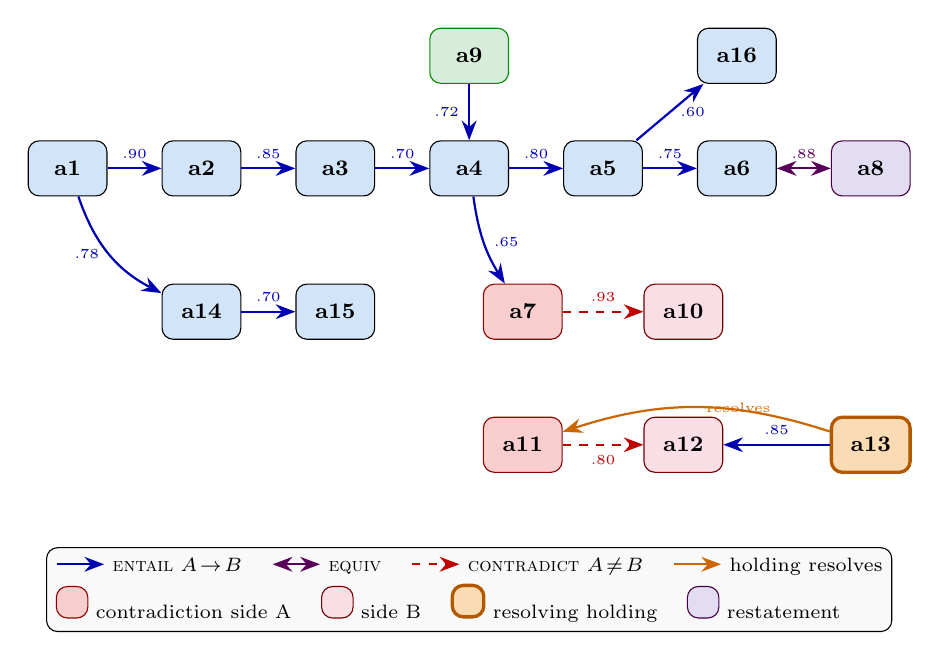
\begin{tikzpicture}[x=17mm,y=13mm]
  % backbone
  \node[unit] (a1) at (0,3)   {a1};
  \node[unit] (a2) at (1,3)   {a2};
  \node[unit] (a3) at (2,3)   {a3};
  \node[unit] (a4) at (3,3)   {a4};
  \node[unit] (a5) at (4,3)   {a5};
  \node[unit] (a6) at (5,3)   {a6};
  \node[equivn](a8) at (6,3)  {a8};
  \node[evid] (a9) at (3,4.1) {a9};
  \node[unit] (a16) at (5,4.1){a16};
  % liability branch
  \node[unit] (a14) at (1,1.6){a14};
  \node[unit] (a15) at (2,1.6){a15};
  % casualty contradiction
  \node[conflA](a7) at (3.4,1.6){a7};
  \node[conflB](a10) at (4.6,1.6){a10};
  % blame contradiction + holding
  \node[conflA](a11) at (3.4,0.3){a11};
  \node[conflB](a12) at (4.6,0.3){a12};
  \node[hold] (a13) at (6,0.3) {a13};

  \draw[prereq] (a1)--node[above,font=\tiny]{.90}(a2);
  \draw[prereq] (a2)--node[above,font=\tiny]{.85}(a3);
  \draw[prereq] (a3)--node[above,font=\tiny]{.70}(a4);
  \draw[prereq] (a4)--node[above,font=\tiny]{.80}(a5);
  \draw[prereq] (a5)--node[above,font=\tiny]{.75}(a6);
  \draw[equivedge] (a6)--node[above,font=\tiny]{.88}(a8);
  \draw[prereq] (a9)--node[left,font=\tiny]{.72}(a4);
  \draw[prereq] (a5)--node[right,font=\tiny]{.60}(a16);
  \draw[prereq] (a4) to[bend right=12] node[right,font=\tiny]{.65}(a7);
  \draw[prereq] (a1) to[bend right=22] node[left,font=\tiny]{.78}(a14);
  \draw[prereq] (a14)--node[above,font=\tiny]{.70}(a15);
  \draw[prereq] (a13)--node[above,font=\tiny]{.85}(a12);

  \draw[invalid] (a7)--node[above,font=\tiny]{.93}(a10);
  \draw[invalid] (a11)--node[below,font=\tiny]{.80}(a12);
  \draw[resolve] (a13) to[bend right=18] node[right,font=\tiny]{resolves}(a11);

  \node[draw,fill=gray!5,rounded corners,anchor=north,align=left,
        font=\scriptsize] at (3,-0.7) {
    \tikz\draw[prereq](0,0)--(6mm,0);~\textsc{entail} $A\!\to\!B$ \quad
    \tikz\draw[equivedge](0,0)--(6mm,0);~\textsc{equiv} \quad
    \tikz\draw[invalid](0,0)--(6mm,0);~\textsc{contradict} $A\!\neq\!B$ \quad
    \tikz\draw[resolve](0,0)--(6mm,0);~holding resolves\\[2pt]
    \tikz\node[conflA,minimum width=4mm,minimum height=4mm]{};~contradiction side A \quad
    \tikz\node[conflB,minimum width=4mm,minimum height=4mm]{};~side B \quad
    \tikz\node[hold,minimum width=4mm,minimum height=4mm]{};~resolving holding \quad
    \tikz\node[equivn,minimum width=4mm,minimum height=4mm]{};~restatement};
\end{tikzpicture}
\end{center}

% =====================================================================================
\section{Relation confidence and uncertainty}
\label{sec:conf}

Each $p_{ij}$ becomes an edge/factor strength. Reuse FactReasoner's two backends
(\texttt{-{}-nli-method}): \textbf{logprobs} (from the generated label's token logprobs;
fast, default) and \textbf{SIMBA-UQ} \citep{simbauq} (self-consistency across sampled
judgments; backend-agnostic, better-calibrated). Two cautions carry extra weight here:
(i) errors compound multiplicatively along a relation chain, so \emph{calibration}
(temperature scaling \citep{calib}) matters more than for single-atom factuality; and
(ii) we need both the \emph{type posterior} $P(\tau_{ij})$ and the \emph{conditional
strength} $P(a_j\mid a_i,\tau_{ij})$ --- their product is the effective $p$ that enters a
factor. If the miner is unsure whether a pair is \textsc{contradict} vs.\ \textsc{none},
that uncertainty should \emph{soften} the contradiction, not be thresholded away.

% =====================================================================================
\section{Model 1 --- Undirected Markov Random Field (FactReasoner-style)}
\label{sec:mrf}

\subsection{Construction (reuses the existing code path)}
Each atom is a binary variable with a unary prior factor $[\,1-\pi,\ \pi\,]$
($\pi=0.5$ for coherence-only; or the factuality FSS for a joint model). Each relation is a
pairwise factor over $[\,\text{src},\text{trg}\,]$, row-major
$(0,0),(0,1),(1,0),(1,1)$. FactReasoner ships \emph{two} table variants
(\texttt{assessor.py::\_edge\_factor\_values}); the choice is the key modeling decision for
coherence.

\begin{center}\small
\renewcommand{\arraystretch}{1.2}
\begin{tabular}{@{}lcc@{}}
\toprule
\textbf{Type} & \textbf{no-priors} (atom$\leftrightarrow$context default)
              & \textbf{with-priors} (recommended for atom$\leftrightarrow$atom)\\
\midrule
\textsc{entail}     & $[\,p,\ p,\ 1{-}p,\ p\,]$ & $[\,1{-}\pi_s,\ \pi_s,\ 1{-}p,\ p\,]$\\
\textsc{contradict} & $[\,p,\ p,\ p,\ 1{-}p\,]$ & $[\,1{-}\pi_s,\ \pi_s,\ p,\ 1{-}p\,]$\\
\textsc{equiv}      & $[\,p,\ 1{-}p,\ 1{-}p,\ p\,]$ & $[\,p,\ 1{-}p,\ 1{-}p,\ p\,]$\\
\bottomrule
\end{tabular}
\end{center}

The joint is $P(\mathbf a)=\tfrac1Z\prod_k f_k(\mathbf a)$; inference is Merlin (WMB,
i-bound 6, MAR task) returning posterior marginals $P(a_i)$; we also request $Z$ (PR task)
for Section~\ref{sec:scoring}.

\subsection*{Modeling finding: use the with-priors variant for coherence}
The no-priors \textsc{entail} table $[\,p,p,1{-}p,p\,]$ penalizes the \emph{source} being
true when the target is uncertain (the $(1,0)$ cell is $1{-}p$). That is desirable for
atom$\leftrightarrow$\emph{context} factuality --- an atom with no supporting context
\emph{should} be pulled down --- but wrong for atom$\leftrightarrow$atom coherence, where a
well-connected \emph{premise} must not be penalized merely for being a premise. Exact
inference confirms it: under the no-priors tables the backbone root a1 collapses to
$P(a1)=0.19$ and mean support is $0.46$ even after \emph{removing} all contradictions. The
with-priors tables decouple the source's own probability from the implication and give the
intended behaviour (Table~\ref{tab:marg}). \textbf{We therefore adopt the with-priors
tables ($\pi_s=0.5$) for atom$\leftrightarrow$atom edges.}

\subsection{Exact marginals on the example}
Table~\ref{tab:marg} gives exact posteriors (brute force over $2^{16}$ worlds) for three
model variants: \textbf{base} (both contradictions active), \textbf{concession-discounted}
(the resolved a11$\neq$a12 softened $0.80\!\to\!0.55$), and a hypothetical
\textbf{coherent rewrite} (all contradictions removed).

\begin{table}[h]\centering\small
\renewcommand{\arraystretch}{1.05}
\begin{tabular}{@{}l*{8}{c}@{}}
\toprule
 & a1 & a2 & a3 & a4 & a5 & a6 & a7 & a8\\
base & .503 & .706 & .761 & .743 & .723 & .681 & \textbf{.612} & .637\\
\midrule
 & a9 & a10 & a11 & a12 & a13 & a14 & a15 & a16\\
base & .531 & \textbf{.237} & .441 & .528 & .441 & .641 & .628 & .572\\
\bottomrule
\end{tabular}
\caption{Exact MRF posterior marginals $P(a_i{=}1)$ for the base model (with-priors
tables, $\pi{=}0.5$). The backbone atoms a2--a6 rise to $0.68$--$0.76$ (well-supported);
the loser of the strong casualty contradiction, \textbf{a10}, is driven to $0.24$; the
softer blame contradiction leaves a11/a12 near $0.44/0.53$.}
\label{tab:marg}
\end{table}

\noindent The \textbf{MAP configuration} (most probable joint world) is the interpretable
"best reading": it sets every backbone atom true, and resolves both contradictions
decisively --- \textbf{a7$=1$, a10$=0$} (accept "no casualties", reject "three died") and
\textbf{a11$=0$, a12$=1$} (reject the retracted pilot-error blame, keep the adjudicated
defect finding), with $P(\mathbf a^*)=4.49\times10^{-3}$.

% =====================================================================================
\section{Model 2 --- Markov Logic Network}
\label{sec:mln}

An MLN \citep{mln,mln-cacm} is a set of weighted first-order formulas $(F_k,w_k)$; grounding
over the atoms yields a Markov network with
$P(\mathbf a)=\tfrac1Z\exp\!\big(\sum_k w_k\,n_k(\mathbf a)\big)$, where $n_k$ counts true
groundings of $F_k$. It was used for textual entailment by \citet{beltagy}. Its advantage
over the pairwise MRF is \emph{expressivity}: relations become first-order rules, and we can
write rules that pairwise factors cannot.

\subsection{Rule schema for coherence}
\begin{align*}
\text{(entail)}\quad & w_e\!\cdot\!p_{ij}:\ \ \mathrm{Entail}(i,j)\wedge a_i \Rightarrow a_j\\
\text{(contradict)}\quad & w_c\!\cdot\!p_{ij}:\ \ \mathrm{Contradict}(i,j)\wedge a_i \Rightarrow \neg a_j\\
\text{(equiv)}\quad & w_q\!\cdot\!p_{ij}:\ \ \mathrm{Equiv}(i,j)\Rightarrow (a_i \Leftrightarrow a_j)\\
\text{(transitivity)}\quad & w_t:\ \ \mathrm{Entail}(i,j)\wedge \mathrm{Entail}(j,k)\Rightarrow \mathrm{Entail}(i,k)\\
\text{(concession cancels)}\quad & w_r:\ \ \mathrm{Resolves}(h,i)\wedge a_h \Rightarrow \neg\,\mathrm{Penalize}(\mathrm{Contradict}(i,j))
\end{align*}
The last two are the point: \textbf{transitivity} lets a weak two-hop chain
(a3$\to$a4$\to$a7) contribute joint evidence a pairwise model treats as independent; the
\textbf{concession-cancels} rule fires on the resolving holding a13 and \emph{removes} the
a11$\neq$a12 penalty when a13 holds --- a first-class treatment of "resolved tension" that
the MRF can only approximate by hand-softening $p$ (the $0.80\!\to\!0.55$ discount of
Section~\ref{sec:mrf}). Higher-arity rules ("an atom contradicted by two independent later
atoms is doubly penalized") are equally expressible.

\subsection{Inference and scoring hooks}
MAP inference (MaxWalkSAT) gives the most-consistent world and its violated-weight energy;
marginal inference (MC-SAT / lifted BP) gives per-atom probabilities analogous to the MRF.
A coherence score is the MAP energy $-\sum_k w_k\,n_k^{\text{viol}}(\mathbf a^*)$ (squashed
to $[0,1]$), or $P(R)$ for a reified rule (Section~\ref{sec:scoring}).

\subsection{MRF vs.\ MLN --- when to use which}
\begin{center}\small
\begin{tabular}{@{}p{3.2cm}p{5.4cm}p{5.4cm}@{}}
\toprule
 & \textbf{MRF (Model 1)} & \textbf{MLN (Model 2)}\\
\midrule
Weights          & $p$ enters factor directly; \emph{no learning} & log-space $w$; needs learning/tuning\\
Cycles / bidir.  & native (undirected) & native (undirected)\\
Expressivity     & pairwise only & full first-order (transitivity, concession-cancel, $n$-ary)\\
Inference cost   & sub-second (Merlin WMB), shipped & \#P-hard; MC-SAT / MaxWalkSAT, new dep.\\
Concession       & hand-softened $p$ & rule that \emph{cancels} the penalty\\
Recommendation   & \textbf{primary} (max reuse, sound) & research branch for rules over relations\\
\bottomrule
\end{tabular}
\end{center}
The MLN is a strict generalization: with only the pairwise (entail/contradict/equiv) rules
and appropriate weights it reproduces the MRF. Adopt the MRF as the default and reach for
the MLN exactly when we need rules \emph{over} relations.

% =====================================================================================
\section{Scoring the coherence of the whole response}
\label{sec:scoring}

We work every applicable readout on the example (base MRF, with-priors). They are not
mutually exclusive; the recommendation is to report the reified-node score with the
$Z$-ratio and mean-support as companions.

\paragraph{S1 --- Joint / geometric-mean product (BN-style, Section~6.1 of the plan).}
The raw joint $\prod$ of relation strengths decays with length; use the length-normalized
geometric mean. Over the 11 \textsc{entail} links the product is $4.19\times10^{-2}$ and the
geometric mean is $\mathbf{0.749}$. \emph{Pro:} intuitive. \emph{Con:} ignores
contradictions unless folded in; needs a DAG for a true joint (cycles here forbid it).

\paragraph{S2 --- Aggregate of posterior marginals (MRF).}
From Table~\ref{tab:marg}: \textbf{mean marginal support} $=0.587$ (base) vs.\ $0.601$
(concession-discounted) vs.\ $0.620$ (coherent rewrite) --- monotone in coherence, as
desired. \textbf{Average normalized entropy} (FactReasoner's $\mathcal E$) $=0.925$ (base),
higher than the coherent rewrite: contradictions push marginals toward $0.5$, raising
entropy. \textbf{Atoms dragged below their prior}: $3$ (base), a crisp diagnostic count
(a10, a11, a13 --- the losers/attachments of the two conflicts).

\paragraph{S3 --- Partition-function ratio (Section~6.3).}
$\mathrm{LCS}=Z_{\text{full}}/Z_{\text{indep}}$, or its log. Here
$\log Z_{\text{base}}=-9.75$ vs.\ $\log Z_{\text{coherent}}=-8.25$: removing the
contradictions raises $Z$ by $\approx\!1.5$ nats --- the structure is "more jointly
satisfiable." This is the most sensitive global signal to contradictions (needs Merlin PR
task) but is not itself in $[0,1]$ without a reference.

\paragraph{S4 --- Reified coherence node $R$ (Section~6.4) --- RECOMMENDED.}
Add one binary $R$ with a factor favouring $R{=}1$ when \textsc{entail}/\textsc{equiv} edges
are satisfied and \textsc{contradict} edges inactive; report $\mathrm{LCS}=P(R{=}1)$. A
single calibrated $[0,1]$ number, length-robust, no DAG needed, one extra factor in the
existing \texttt{MarkovNetwork}. This is the clean bridge from per-atom marginals to an
argument-level score.

\paragraph{S5 --- MAP energy / PSL satisfaction (Section~6.5).}
MRF/MLN: report the MAP world and its (normalized) probability $P(\mathbf a^*)=4.49\times
10^{-3}$, or the count of violated relations at the MAP world ($1$: the unresolved a7/a10).
PSL \citep{psl} gives $1-\text{mean distance-to-satisfaction}$ directly in $[0,1]$.

\paragraph{S6 --- $\alpha/\beta$ support-vs-contradiction knob (Section~6.6).}
$\mathrm{LCS}=\sigma\!\big((\alpha\sum_{\text{ent}}p - \beta\sum_{\text{con}}p)/|E|\big)$
with $\beta>\alpha$ penalizing contradictions harder. With support mass $S=9.18$,
contradiction mass $C=1.73$: $(\alpha,\beta)=(1,1)\!\to\!0.630$; $(1,2)\!\to\!0.601$;
$(1,3)\!\to\!0.571$. A cheap post-hoc layer to calibrate on human ratings, usable atop any
core score.

\begin{table}[h]\centering\small
\begin{tabular}{@{}llccc@{}}
\toprule
 & \textbf{Readout} & \textbf{base} & \textbf{concession-disc.} & \textbf{coherent rewrite}\\
\midrule
S1 & geo-mean of \textsc{entail} $p$      & 0.749 & 0.749 & 0.749\\
S2 & mean marginal support               & 0.587 & 0.601 & 0.620\\
S2 & avg.\ normalized entropy $\downarrow$& 0.925 & --    & lower\\
S3 & $\log Z_{\text{full}}$               & $-9.75$ & $-9.42$ & $-8.25$\\
S5 & MAP prob $P(\mathbf a^*)$            & $4.5\!\times\!10^{-3}$ & -- & --\\
S6 & $\sigma$, $(\alpha,\beta)=(1,2)$     & 0.601 & -- & --\\
\bottomrule
\end{tabular}
\caption{All applicable scoring readouts on the worked example. S1 (relation-only) is
blind to contradictions --- it cannot tell the three variants apart --- which is exactly why
S2/S3/S4 (inference-based) are preferred: they \emph{decrease} for the contradiction-laden
base and \emph{recover} as tensions are resolved or removed.}
\label{tab:scores}
\end{table}

\subsection{Scoring-behavior figure}
Figure~\ref{fig:scoring} plots the two inference-based global scores (mean support, and
$\log Z$ rescaled) across the three variants, against the contradiction-blind S1 baseline.

\begin{figure}[h]\centering
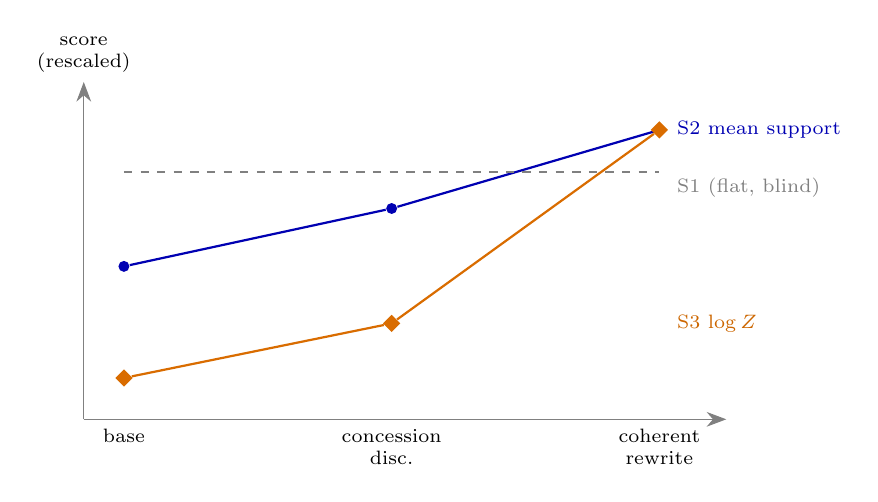
\begin{tikzpicture}[x=34mm,y=42mm]
  \draw[->,gray] (-0.15,0)--(2.25,0);
  \draw[->,gray] (-0.15,0)--(-0.15,1.02) node[above,font=\scriptsize,black,align=center]{score\\(rescaled)};
  \foreach \x/\lab in {0/base, 1/{concession\\disc.}, 2/{coherent\\rewrite}}
    \node[font=\scriptsize,align=center,below] at (\x,0) {\lab};
  % mean support (0.587,0.601,0.620) rescale to [0,1] over window [0.55,0.63]
  \def\sA{0.4625}\def\sB{0.6375}\def\sC{0.875}
  \node[circle,fill=blue!70!black,inner sep=1.4pt] (mA) at (0,\sA){};
  \node[circle,fill=blue!70!black,inner sep=1.4pt] (mB) at (1,\sB){};
  \node[circle,fill=blue!70!black,inner sep=1.4pt] (mC) at (2,\sC){};
  \draw[blue!70!black,thick] (mA)--(mB)--(mC);
  \node[font=\scriptsize,blue!70!black,right] at (2.03,\sC){S2 mean support};
  % logZ (-9.75,-9.42,-8.25) rescale over [-10,-8]
  \def\zA{0.125}\def\zB{0.29}\def\zC{0.875}
  \node[diamond,fill=orange!85!black,inner sep=1.6pt] (zA) at (0,\zA){};
  \node[diamond,fill=orange!85!black,inner sep=1.6pt] (zB) at (1,\zB){};
  \node[diamond,fill=orange!85!black,inner sep=1.6pt] (zC) at (2,\zC){};
  \draw[orange!85!black,thick] (zA)--(zB)--(zC);
  \node[font=\scriptsize,orange!80!black,right] at (2.03,\zB){S3 $\log Z$};
  % S1 flat baseline (0.749) constant
  \draw[gray,dashed,thick] (0,0.749)--(2,0.749);
  \node[font=\scriptsize,gray,right] at (2.03,0.70){S1 (flat, blind)};
\end{tikzpicture}
\caption{Global coherence scores across the three variants (higher $=$ more coherent).
The inference-based scores S2 (mean marginal support) and S3 ($\log Z$) rise as
contradictions are resolved/removed; the relation-only baseline S1 is flat because it never
sees the contradictions. Values are those of Table~\ref{tab:scores}, each linearly rescaled
to a common axis for shape comparison.}
\label{fig:scoring}
\end{figure}

% =====================================================================================
\section{Synthesis and recommendations}
\label{sec:synthesis}

\begin{enumerate}[leftmargin=*]
  \item \textbf{Taxonomy.} Adopt the two-layer scheme: mine an interpretable PDTB/RST
        \emph{discourse} sense, map it to an \textsc{entail}/\textsc{contradict}/\textsc{equiv}
        \emph{coupling} with a graded strength. Treat Concession / adjudicated holdings as
        \emph{resolved} tensions, not defects.
  \item \textbf{Primary model: the pairwise MRF} (Model 1), reusing
        \texttt{MarkovNetwork}\,$+$\,Merlin, \textbf{with the \emph{with-priors} factor
        tables} for atom$\leftrightarrow$atom edges (the no-priors tables mis-penalize
        premises --- Section~\ref{sec:mrf}). This is a small delta on shipped code:
        add \texttt{link="atom\_atom"} edges and one reified factor.
  \item \textbf{Research branch: the MLN} (Model 2) when we need rules \emph{over} relations
        --- transitivity of entailment and, especially, a concession-cancels-penalty rule
        that the MRF can only approximate by hand-softening $p$.
  \item \textbf{Primary score: the reified coherence node} $P(R{=}1)$ (S4), reported with
        \textbf{mean marginal support} (S2) and the \textbf{$\log Z$ ratio} (S3) as
        companions. Avoid relation-only products (S1) as the headline number --- they are
        blind to contradictions (Table~\ref{tab:scores}). Keep the $\alpha/\beta$ knob (S6)
        as a calibration layer.
  \item \textbf{Evaluation.} Unit-test the miner and the scores on the five ideation PDFs
        plus this example; stress order-sensitivity on \emph{Renda} S vs.\ K; correlate
        against human coherence ratings, benchmarking DiscoScore \citep{discoscore} and a
        G-Eval \citep{geval} LLM-judge; ablate logprobs vs.\ SIMBA-UQ and with/without
        calibration.
\end{enumerate}

\paragraph{Reproducibility.} All marginals, $Z$, and MAP values in
Sections~\ref{sec:mrf}--\ref{sec:scoring} are exact (brute force over $2^{16}$ worlds) for
the model of Section~\ref{sec:example} using the with-priors factor tables of
\texttt{assessor.py}; they are intended to be regenerated by a small reference solver as
the design is prototyped against Merlin.

% =====================================================================================
\begin{thebibliography}{99}\small
\bibitem[FactReasoner]{factreasoner} R.~Marinescu et al.
  \emph{FactReasoner: A Probabilistic Approach to Long-Form Factuality Assessment for LLMs.}
  arXiv:2502.18573, 2025.
\bibitem[SIMBA-UQ]{simbauq} D.~Bhattacharjya et al.
  \emph{SIMBA-UQ: Similarity-Based Aggregation for UQ in LLMs.} Findings of EMNLP 2025,
  arXiv:2510.13836.
\bibitem[PDTB3]{pdtb3} B.~Webber, R.~Prasad, A.~Lee, A.~Joshi.
  \emph{The Penn Discourse Treebank 3.0 Annotation Manual.} LDC2019T05, 2019.
\bibitem[PDTB2]{pdtb2} R.~Prasad et al. \emph{The Penn Discourse TreeBank 2.0.} LREC 2008.
\bibitem[RST]{rst} W.~Mann, S.~Thompson. \emph{Rhetorical Structure Theory.} Text 8(3), 1988.
\bibitem[SDRT]{sdrt} N.~Asher, A.~Lascarides. \emph{Logics of Conversation.} CUP, 2003.
\bibitem[DiscoPrompt]{discoprompt} C.~Chan et al.
  \emph{DiscoPrompt: Path Prediction Prompt Tuning for Implicit Discourse Relation
  Recognition.} ACL Findings 2023, arXiv:2305.03973.
\bibitem[MLN]{mln} M.~Richardson, P.~Domingos. \emph{Markov Logic Networks.}
  Machine Learning 62, 2006.
\bibitem[Markov Logic]{mln-cacm} P.~Domingos et al.
  \emph{Unifying Logical and Statistical AI with Markov Logic.} CACM 62(7), 2019.
\bibitem[RTE-MLN]{beltagy} I.~Beltagy, K.~Erk.
  \emph{Representing Meaning with a Combination of Logical and Distributional Models.}
  Computational Linguistics, 2016, arXiv:1505.06816.
\bibitem[PSL]{psl} S.~Bach, M.~Broecheler, B.~Huang, L.~Getoor.
  \emph{Hinge-Loss Markov Random Fields and Probabilistic Soft Logic.} JMLR 18(109), 2017,
  arXiv:1505.04406.
\bibitem[WMC]{wmc} M.~Chavira, A.~Darwiche.
  \emph{On Probabilistic Inference by Weighted Model Counting.} AIJ 172(6--7), 2008.
\bibitem[Calib]{calib} C.~Guo et al. \emph{On Calibration of Modern Neural Networks.}
  ICML 2017.
\bibitem[DiscoScore]{discoscore} W.~Zhao, M.~Strube, S.~Eger.
  \emph{DiscoScore.} EACL 2023, arXiv:2201.11176.
\bibitem[G-Eval]{geval} Y.~Liu et al. \emph{G-Eval: NLG Evaluation using GPT-4.}
  EMNLP 2023, arXiv:2303.16634.
\end{thebibliography}

\end{document}
